\documentclass[11pt]{beamer}
\usetheme{Warsaw}
\usepackage[utf8]{inputenc}
\usepackage[french]{babel}
\usepackage[T1]{fontenc}
\usepackage{amsmath}
\usepackage{amsfonts}
\usepackage{amssymb}
\usepackage{graphicx}
\usepackage{tikz}
\setbeamertemplate{navigation symbols}{}

%%%%%%%%%%%%%%%%%%%%%%%%%%%%%%%%%%%%%%%%%%%%%%%%%%%%%%%%%
\author{Théophile \textsc{Bastian}, Kévin \textsc{Le Run}, Rémi \textsc{Oudin}}
\title{HPP \& \og{}Hilare pulling a trailer~\fg}
\date{24 janvier 2017}
%\subject{}
%\logo{}
%\institute{}
\begin{document}

\begin{frame}
	\titlepage{}
	\tableofcontents
\end{frame}

%\begin{frame}
%\tableofcontents
%\end{frame}

\section{Problèmes d'installation de HPP}

\subsection{Installation de ROS}

\begin{frame}
    \frametitle{\subsecname}
    \begin{itemize}
        \item Une partie de ROS indigo en dépendance obligatoire.
        \item Indigo est actuellement la version \emph{Old Old Stable} de ROS\@.
        \item Ne fonctionne que sous Ubuntu 12.04 et 14.04
        \item Toute autre distribution est soit expérimentale soit trop moderne
        \item Pas de support pour les versions récentes de Debian
        \item L'installation sous Arch et Xubuntu n'est pas non plus
            fonctionnelle
    \end{itemize}
\end{frame}

\subsubsection{Solutions?}

\begin{frame}
    \frametitle{\subsecname}
    \begin{enumerate}
        \item Essayé nos machines
        \item Essayé sur un serveur Debian Jessie. ROS ok mais pas HPP\@.
        \item Essayé sur un serveur Ubuntu 12.04. ROS et HPP ok.
    \end{enumerate}
\end{frame}

\section{Architecture de HPP}

\begin{frame}
    \begin{figure}
        \begin{center}
            \begin{tikzpicture}
                \node at (0,1)
                {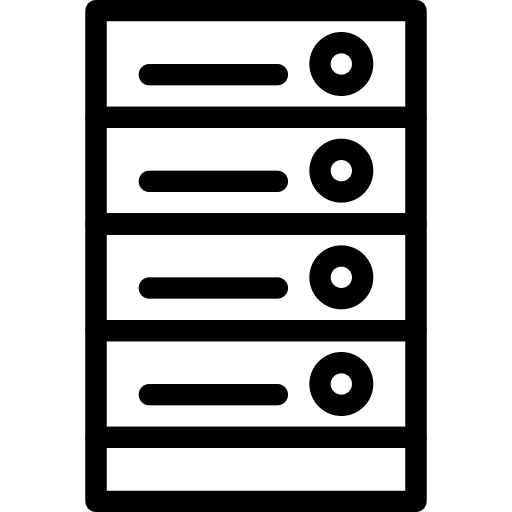
\includegraphics[width=0.1\textwidth]{server_icon.png}};
                \node[rectangle, draw] (c) at (0,0) {CORBA};
                \onslide<2->{%
                    \node[rectangle, draw] (r) at (4,2) {Robots};
                    \node[rectangle, draw] (o) at (4,0) {Obstacles};
                    \node[rectangle, draw] (p) at (4,-2) {Problèmes};
                    \draw[->] (c) edge (r) (c) edge (o) (c) edge (p);
                }
                \onslide<3->{%
                    \node[rectangle, draw] (c1) at (-4,1) {Client};
                    \node at (-4,0) {$\vdots$};
                    \node[rectangle, draw] (c2) at (-4,-1) {Client};
                    \draw[->] (c1) edge (c) (c2) edge (c);
                }
            \end{tikzpicture}
        \end{center}
    \end{figure}
\end{frame}
\end{document}
